\documentclass[a4paper,11pt]{beamer}
\usepackage{etex}
\usepackage{lmodern}
\usepackage[french]{babel}
\usepackage[T1]{fontenc}
\usepackage[utf8]{inputenc}
% \usepackage{listings}
\usepackage{graphicx} 
\usepackage{ragged2e}
\usepackage{enumitem}
\usepackage{array}
% \usepackage{tikz} 
% \usepackage{pgf-umlcd} 
% \usepackage{csquotes}
\usepackage{pst-sigsys}
\usepackage{amsmath,amsfonts,bm}
\usepackage{pstricks-add}
% \usepackage{physics}
% \usepackage{ulem}
% \usepackage{wasysym}
\usepackage{hyperref}
% \usepackage{color}
\usepackage{matlab-prettifier} 
\usepackage{comment} 


\setenumerate{label*=\arabic*.} 

\setbeamertemplate{navigation symbols}{}  
  
\usetheme{Darmstadt} 
\setbeamertemplate{footline}{\insertframenumber/\inserttotalframenumber}
\title{L3 - CMI017 : Signaux et Systèmes\\Séquence II}
\author{BULOUP Frank}
\institute{Aix Marseille Université\\Institut des Sciences du Mouvement}
\date{}

\setbeamertemplate{footline} 
{  
	\begin{beamercolorbox}[ht=2.5ex,dp=1.125ex,%
      leftskip=.3cm,rightskip=.3cm plus1fil]{title in head/foot}%
      {\usebeamerfont{title in head/foot}\insertshorttitle} \hfill    
      \insertframenumber / \inserttotalframenumber%
    \end{beamercolorbox}%
%     \begin{beamercolorbox}[colsep=1.5pt]{lower separation line foot}
%     \end{beamercolorbox} 
}

\newcounter{exampleBlockCounter}
\setcounter{exampleBlockCounter}{1}

\definecolor{comment}{rgb}{0.12, 0.38, 0.18 } %adjusted, in Eclipse: {0.25, 0.42, 0.30 } = #3F6A4D
\definecolor{keyword}{rgb}{0.37, 0.08, 0.25}  % #5F1441
\definecolor{string}{rgb}{0.06, 0.10, 0.98} % #101AF9
\definecolor{myGreen}{rgb}{0,0.4,0}

% \lstset {language=Java,
%  frame=single,
%  frameround=tttt,
%  rulesepcolor=\color{black},
%  showspaces=false,showtabs=false,tabsize=2,
%  numberstyle=\tiny,numbers=left,
%  stringstyle=\color{string},
%  keywordstyle = \color{keyword}\bfseries,
%  commentstyle=\color{comment}\itshape,
%  basicstyle=\ttfamily\footnotesize,
%  breaklines=true,
%  captionpos=b
% }

% \renewenvironment{package}[2][\umlcdPackageTitle]{
% \edef\umlcdPackageTitle{#2}
% \def\umlcdPackageFit{}
% \def\umlcdPackageName{#1}
% }{
%   \begin{pgfonlayer}{background}
%   \node[umlcd style, draw, inner sep=0.5cm, fit = \umlcdPackageFit] (\umlcdPackageName) {};
%   \node[umlcd style, draw, outer ysep=-0.5, anchor=south west] (\umlcdPackageName caption) at
%   (\umlcdPackageName.north west) {\umlcdPackageTitle};
%   \end{pgfonlayer}
% }

\begin{document}

\begin{frame}[plain]  
	\titlepage  
	\center{\includegraphics[scale=0.75]{images/by-nc-sa.eps}}
	\vspace{1cm}
	
	\includegraphics[scale=0.6]{images/LogoAMU.png}\hspace*{2cm}
	\includegraphics[scale=0.2]{images/LogoCNRS.eps}\hspace*{2cm}
	\includegraphics[scale=0.1]{images/LogoISM.eps}
\end{frame} 
  

\begin{frame}{Plan de cette séquence}
	\tableofcontents[hideallsubsections]
\end{frame}

\AtBeginSection[]{
\begin{frame}{Signaux et Systèmes}
	\tableofcontents[currentsection,hideallsubsections]
\end{frame}
}

\begin{comment}

\begin{frame}{Rappels 1/3}
\begin{alertblock}{Rappel I}
\justifying
Les hypothèses de linéarité et d'invariance temporelle d'un système permettent
d'obtenir une relation temporelle E/S générique : convolution entre entrée et réponse
impulsionnelle du système.
\end{alertblock}
\pause
\begin{alertblock}{Rappel II}
\justifying
La fonction de transfert en z d'un SDLIT s'obtient en remplaçant $\mathcal{R}$
par $z^{-1}$ dans la fonction de transfert en $\mathcal{R}$.
\end{alertblock}
\pause
\begin{alertblock}{Rappel III}
\justifying
La TZ de la réponse impulsionnelle d'un SDLIT est sa fonction de transfert en
$z$.
\end{alertblock}
\end{frame}

\begin{frame}{Rappels 2/3}
\begin{alertblock}{Rappel IV}
\justifying
Généralement, la fonction de transfert en $z$ d'un SDLIT est une fonction
rationnelle de la variable $z$ et possède, à ce titre, des zéros et des pôles :
\begin{enumerate}
  \item le système est alors bouclé, on dit aussi récursif, et sa réponse
  impulsionnelle est infinie
  \item si les modules des pôles sont inférieurs à un, le système est stable
\end{enumerate}
\end{alertblock}
\end{frame}

\begin{frame}{Rappels 3/3}
\begin{alertblock}{Rappel V}
\justifying
Si la fonction de transfert en $z$ ne possède pas de dénominateur, donc pas de
pôles :
\begin{enumerate}
  \item le système est non bouclé, on dit aussi non récursif, et sa réponse
  impulsionnelle est finie
  \item le système est toujours stable
\end{enumerate}
\end{alertblock}
\end{frame}
\end{comment}

\section[Rep. des phénomènes périodiques]{Représentations des phénomènes
périodiques}
\subsection{Représentation temporelle}

\begin{frame}
\begin{block}{Phénomène périodique élémentaire}
La cosinusoïde est le phénomène périodique le plus simple :
$$x(t) = Acos(2\pi f_0 t + \phi)$$
Avec :
\begin{itemize}[label=$\bullet$]
  \item $A$ : l'amplitude de l'oscillation
  \item $\phi$ : la phase en $rad$
  \item $\omega_0=2\pi f_0$ : pulsation (fréquence angulaire) en $rad\cdot
  s^{-1}$
  \item $f_0$ : la fréquence en $Hz$. $f_0 = \frac{1}{T_0}$, $T_0$ étant la
  période en $s$
\end{itemize}
\end{block}
\pause
\begin{alertblock}{Phénomène périodique plus complexe}
\begin{itemize}[label=$\bullet$]
  \item superposition de phénomènes périodiques élémentaires
  \item les fréquences sont des multiples d'une fréquence de référence
  \item Cette fréquence est appelée la fondamentale
\end{itemize}
\end{alertblock}
\end{frame}

\begin{frame}
\begin{block}{Remarque}
\justify
Une superposition de phénomènes périodiques élémentaires n'est pas forcément
périodique. Par exemple :
$$
x(t) = cos(2x) + cos(\pi x)
$$ 
\justify
n'est pas périodique parce qu'il n'existe pas d'entiers $p$ et $q$ tels que :
$$
p\times 2 = q\times \pi
$$
\justify
puisque $\pi$ est irrationnel.
\end{block}
\end{frame}

\begin{frame}
\begin{block}{Autre notation}
$$
\begin{aligned}
x(t) = Acos(2\pi f t + \phi) &= \Re[A e^{i(2\pi ft +\phi)}]\\
& =\frac{A e^{i(2\pi ft + \phi)} + A e^{-i(2\pi ft+ \phi)}}{2} 
\end{aligned}
$$
Puisque :
$$
e^{\pm i\theta} = cos(\theta) \pm i\cdot sin(\theta)
$$
\end{block}
\end{frame}

\begin{frame}
\begin{block}{Série de Fourier - Cas général}
\justify
Presque tout signal périodique, noté $x(t)$, peut être décomposé en
superposition de « cosinusoïdes » :
$$x(t) = \sum_{k=-\infty}^{+\infty}X(k)e^{2i\pi kf_0 t}$$ 
\justify
Les paramètres de cette décomposition sont donnés par le calcul de l'intégrale
suivante :
$$X(k) = \frac{1}{T_0}\int_{T_0} x(t)e^{-2i\pi kf_0 t}dt$$
\end{block}
\end{frame}

\begin{frame}
\begin{exampleblock}{Exercice \Roman{exampleBlockCounter} - Propriétés de la
Série de Fourier lorsque $x(t)$ est réel}
\justifying
On supposera maintenant et dans toute la suite du cours que $x(t)$ est réel.
$X(k)$ est un nombre complexe que l'on peut noter de la façon suivante :
$$
X(k) = \rho(k) e^{i\phi(k)}
$$ 
Avec :
\begin{itemize}[label=$\bullet$]
  \item $\rho(k) = \lvert X(k) \rvert$, le module.
  \item $\phi(k) = arg[X(k)]$, la phase.
\end{itemize}
\begin{enumerate}
  \item Quelle est l'expression de $X(0)$ ? Commentez.
  \item Quelles propriétés vérifient $\rho(k)$ et $\phi(k)$ lorsque $x(t)$ est
  réel ?
  \item Proposez alors une autre écriture de $x(t)$ en fonction de $\rho(k)$ et
  $\phi(k)$ qui ne prenne en compte que les fréquences positives ou nulle
  ($k\geq 0$).
\end{enumerate}
  
\end{exampleblock}
\end{frame}
\stepcounter{exampleBlockCounter}

\begin{frame}[containsverbatim]
\begin{exampleblock}{Exercice
\Roman{exampleBlockCounter} - Synthèse d'un
signal triangulaire}\stepcounter{exampleBlockCounter} Avec Matlab créez un
script et collez le code suivant dedans :
\begin{lstlisting}[style=Matlab-editor]
clear all; close all; clc;
time = 0:.001:2;
x = 0;
for k = 0:2
    rho = 4/((2*k+1)*pi)^2; phi = -pi; 
    x = x+2*rho*cos(2*pi*(2*k+1)*time+phi);    
    plot(time, x);
    title(['k = ', int2str(k)]);
    xlabel('time'); ylabel('x(t)');
    pause(0.15);
end
\end{lstlisting}
Augmentez le nombre de termes de la série et concluez.
\end{exampleblock}
\end{frame}

\begin{frame}[containsverbatim]
\begin{exampleblock}{Exercice
\Roman{exampleBlockCounter} - Synthèse d'un
signal carré}\stepcounter{exampleBlockCounter}
Avec Matlab créez un script et collez le code suivant dedans :
\begin{lstlisting}[style=Matlab-editor]
clear all; close all; clc;
time = 0:.001:2;
x = 0;
for k = 0:2
    rho = 2/((2*k+1)*pi); phi = -pi/2; 
    x = x+2*rho*cos(2*pi*(2*k+1)*time+phi);    
    plot(time, x);
    title(['k = ', int2str(k)]);
    xlabel('time'); ylabel('x(t)');
    pause(0.15);
end
\end{lstlisting}
Augmentez le nombre de termes de la série et concluez.
\end{exampleblock}
\end{frame}

\begin{frame}
\begin{alertblock}{Phénomène de GIBBS}
\justify
Si le signal comporte des discontinuités, des oscillations apparaissent autour
de celles-ci sans diminuer en amplitude avec l'augmentation du
nombre de termes de la série.
\href{http://en.wikipedia.org/wiki/Gibbs_phenomenon}{\underline{En savoir
plus}}.
\center
\includegraphics [width=2.25in]{images/Exercice_III_01.eps} 
\vspace{\baselineskip}
\end{alertblock}
\end{frame}


\subsection{Représentation fréquentielle}
\begin{frame}
\begin{block}{Spectres d'un signal périodique}
\justify
On peut représenter le nombre complexe $X(k)$ associé à $x(t)$ sous la forme de
deux graphes :
\begin{itemize}[label=$\bullet$]
  \item \alert{Spectre d'amplitude} : on représente $\lvert X(k) \rvert$ en
  fonction de $kf_0$
  \item \alert{Spectre de phase} : on représente $arg[X(k)]$ en fonction de
  $kf_0$
\end{itemize}
On peut tracer ces \alert{spectres} sur les fréquences positives uniquement.
Dans ce cas ils sont qualifiés de \alert{monolatéraux}. Si on les trace sur tout
le support fréquentiel, ils sont dits \alert{bilatéraux}.
\end{block}
\end{frame}

\begin{frame}
\begin{alertblock}{Spectre d'amplitude}
\center
lié à l'amplitude $\Leftrightarrow$ répartition énergétique\\
\alert{\textbf{Quelles sont les oscillations élémentaires\\ porteuses d'énergie
?}}
\end{alertblock}
\pause
\begin{alertblock}{Spectre de phase}
\center
lié à la phase $\Leftrightarrow$ répartition temporelle\\
\alert{\textbf{De quelle façon doivent se recombiner ces oscillations
élémentaires significatives pour reconstituer le signal ?}}\\
La phase contient toute l'information temporelle\\
Elle est plus difficile à interpréter et à mettre en oeuvre
\end{alertblock}
\end{frame}

\begin{frame}
\center
\includegraphics [width=3.75in]{images/RepSpectrale_01.eps}
\end{frame}

\begin{frame}
\center
\includegraphics [width=3.75in]{images/RepSpectrale_02.eps} 
\end{frame}

% \section[Rep. des phénomènes transitoires]{Représentation des phénomènes
% transitoires}
% \subsection{Phénomène transitoire et Transformée de Fourier}
% \begin{frame}
% \center
% Mais bien souvent, on souhaite analyser des phénomènes
%  \textbf{\alert{transitoires, apériodiques ou encore d'énergie finie}} !
%  
% \vspace{2\baselineskip}
% Comment fait-on dans ce cas ?
% 
% \vspace{2\baselineskip}
% \pause
% \textbf{\alert{$\Rightarrow$ Transformée de Fourier}}
% \end{frame}
% 
% \begin{frame}
% \begin{block}{Transformée de Fourier}
% \justify
% Presque tout signal transitoire, noté $x(t)$, admet une transformée de Fourier :
% $$X(f) = \int_{-\infty}^{+\infty}x(t)e^{-2i\pi ft}dt$$ 
% \justify
% On retrouve le signal original par la transformée inverse :
% $$x(t) = \int_{-\infty}^{+\infty}X(f)e^{2i\pi ft}df$$ 
% \justify
% Comme pour la série de Fourier, $X(f)$ est un nombre complexe :
% \begin{itemize}[label=$\bullet$]
%   \item $\rho(f) = \lvert X(f) \rvert$, le module
%   \item $\phi(f) = arg[X(f)]$, la phase
% \end{itemize}
% \center
% \alert{
% \textbf{Le support fréquentiel est maintenant continu sur
% $\mathbb{R}$}}
% \end{block}
% \end{frame}
% 
% \begin{frame}
% \begin{block}{Remarques}
% \justify
% \begin{itemize}[label=$\bullet$]
%   \item La transformée de fourier est une généralisation de la série de Fourier
%   \item Les signaux périodiques admettent une transformée de Fourier qui se
%   trouve être équivalente à la série de Fourier
% \end{itemize} 
% \end{block}
% \end{frame} 

\section[La TFD]{La Transformée de Fourier Discrète}
\subsection{Situation réelle et Transformée de Fourier Discrète}
\begin{frame}
\begin{block}{Situation réelle}
\justify
On acquière sur ordinateur un signal pendant une durée
finie $D = (N-1)T_e$, $N$ étant le nombre d'échantillons et $T_e$ la période
d'échantillonnage. 
\end{block}
\begin{exampleblock}{Exercice \Roman{exampleBlockCounter} -
Résolution de TFD}
\center
Quelle sera alors la plus petite fréquence observable ?
\pause
\center
\includegraphics [width=1.5in]{images/Exercice_IV_01.eps}
\pause 
$$\Delta f=\frac{1}{NT_e}\text{ à comparer à }f_0\text{ dans la série de
Fourier}$$
\end{exampleblock}
\end{frame}
\stepcounter{exampleBlockCounter}

\begin{frame}
\begin{block}{Transformée de Fourier Discrète}
\justify
En partant des observations précédentes, on peut en
déduire la formulation discrète de la série de Fourier :
$$
\begin{aligned}
X(kf_0) &= \frac{1}{T_0}\int_{T_0} x(t) e^{-2i\pi kf_0 t}dt \\
X(k\Delta f) &= \frac{1}{NT_e}\sum_{n=0}^{N-1}x(nT_e)e^{-2i\pi k
\frac{1}{NT_e}nT_e}T_e\\
X(k\Delta f) &= \frac{1}{N}\sum_{n=0}^{N-1}x(nT_e)e^{-2i\pi
\frac{kn}{N}}
\end{aligned}
$$ 
\center
Avec $\Delta f=\frac{1}{NT_e}$, résolution fréquencielle de la TFD
\end{block}
\end{frame}

\subsection{Lien avec la transformée en z}
\begin{frame}
\justifying
On peut réécrire cette TFD de la façon suivante :
$$
X(k) = \frac{1}{N}\sum_{n=0}^{N-1}x(n)e^{-2i\pi\frac{kn}{N}}
$$
et en posant $z = e^{2i\pi\frac{k}{N}}$, son expression devient :
$$
X(z) = \frac{1}{N}\sum_{n=0}^{N-1}x(n)z^{-n}
$$
qui est, au facteur $\frac{1}{N}$ près, la TZ de $x(n)$
\end{frame}

\subsection{Illustration : FFT d'une cosinusoïde}
\begin{frame}
\begin{block}{Transformée de Fourier Rapide, TFR}
\center
La TFR est une algorithme optimisé de la TFD
\end{block}
\begin{exampleblock}{Exercice \Roman{exampleBlockCounter} - Spectre d'amplitude
d'un signal avec Matlab}
\justify
On a acquis $100$ échantillons du signal suivant : 
$$
x(t) = 2\cdot cos(2\pi 100 t) + \frac{1}{2}cos(2\pi 200 t) + cos(2\pi 250 t)
$$ 
avec un pas d'échantillonnage de $1ms$.
\begin{enumerate}
  \item Simuler cette acquisition dans un script Matlab.
  \item Utiliser les fonctions \textbf{fft} et \textbf{fftshift} pour calculer
  la TFR de ce signal.
  \item Calculer \textbf{magFFTX}, le module de cette TFR (utiliser
  \textbf{abs}).
  \item Créer le vecteur fréquenciel pour une représentation bilatérale. 
  \item Tracer le spectre d'amplitude (utiliser la fonction \textbf{stem}).
\end{enumerate}
\end{exampleblock}
\end{frame}
\stepcounter{exampleBlockCounter}

\section{Home work !}
\begin{frame}
\begin{exampleblock}{Exercice \Roman{exampleBlockCounter} - Calculs de séries
de Fourier}
\justifying
Pour les signaux triangulaire et carré ci-après :
\begin{enumerate}
  \item Calculer les coefficients complexes des séries de Fourier associées.
  \item Tracer les spectres d'amplitude et de phase correspondants.
\end{enumerate} 
\end{exampleblock}
\end{frame}
 
\begin{frame}
\begin{exampleblock}{Exercice \Roman{exampleBlockCounter} - Calculs de séries
de Fourier}
\centering
Signal triangulaire :
\vspace{0.25cm}

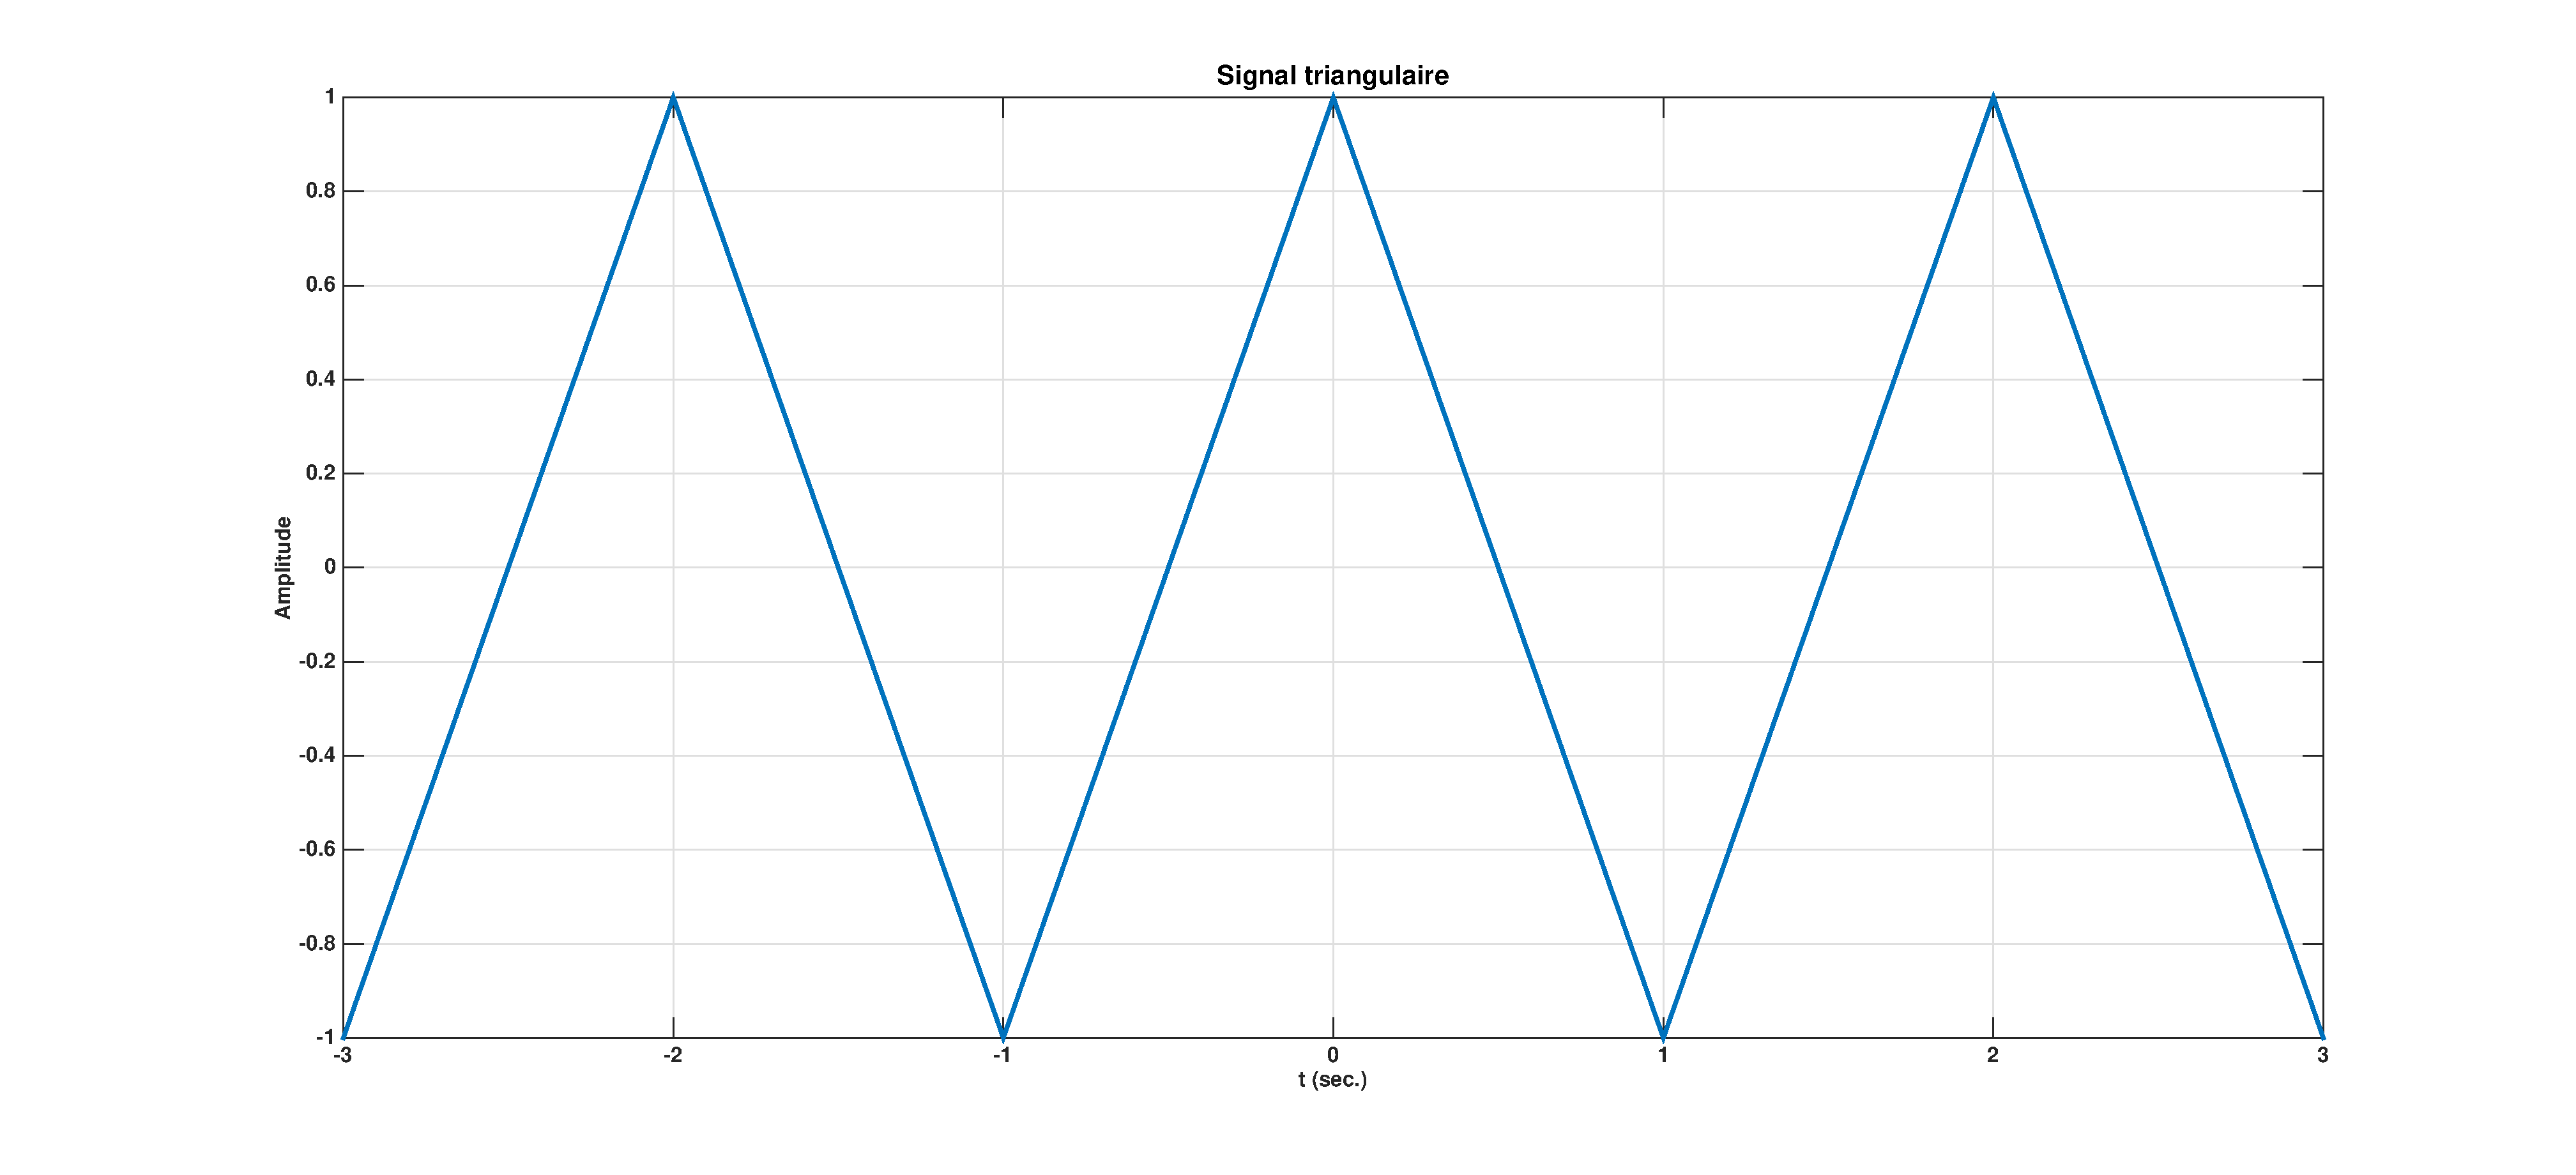
\includegraphics[scale=0.15]{Matlab/SignalTriangulaire.eps}
\end{exampleblock}
\end{frame}
 
\begin{frame}
\begin{exampleblock}{Exercice \Roman{exampleBlockCounter} - Calculs de séries
de Fourier}
\centering
Signal carré :
\vspace{0.25cm}

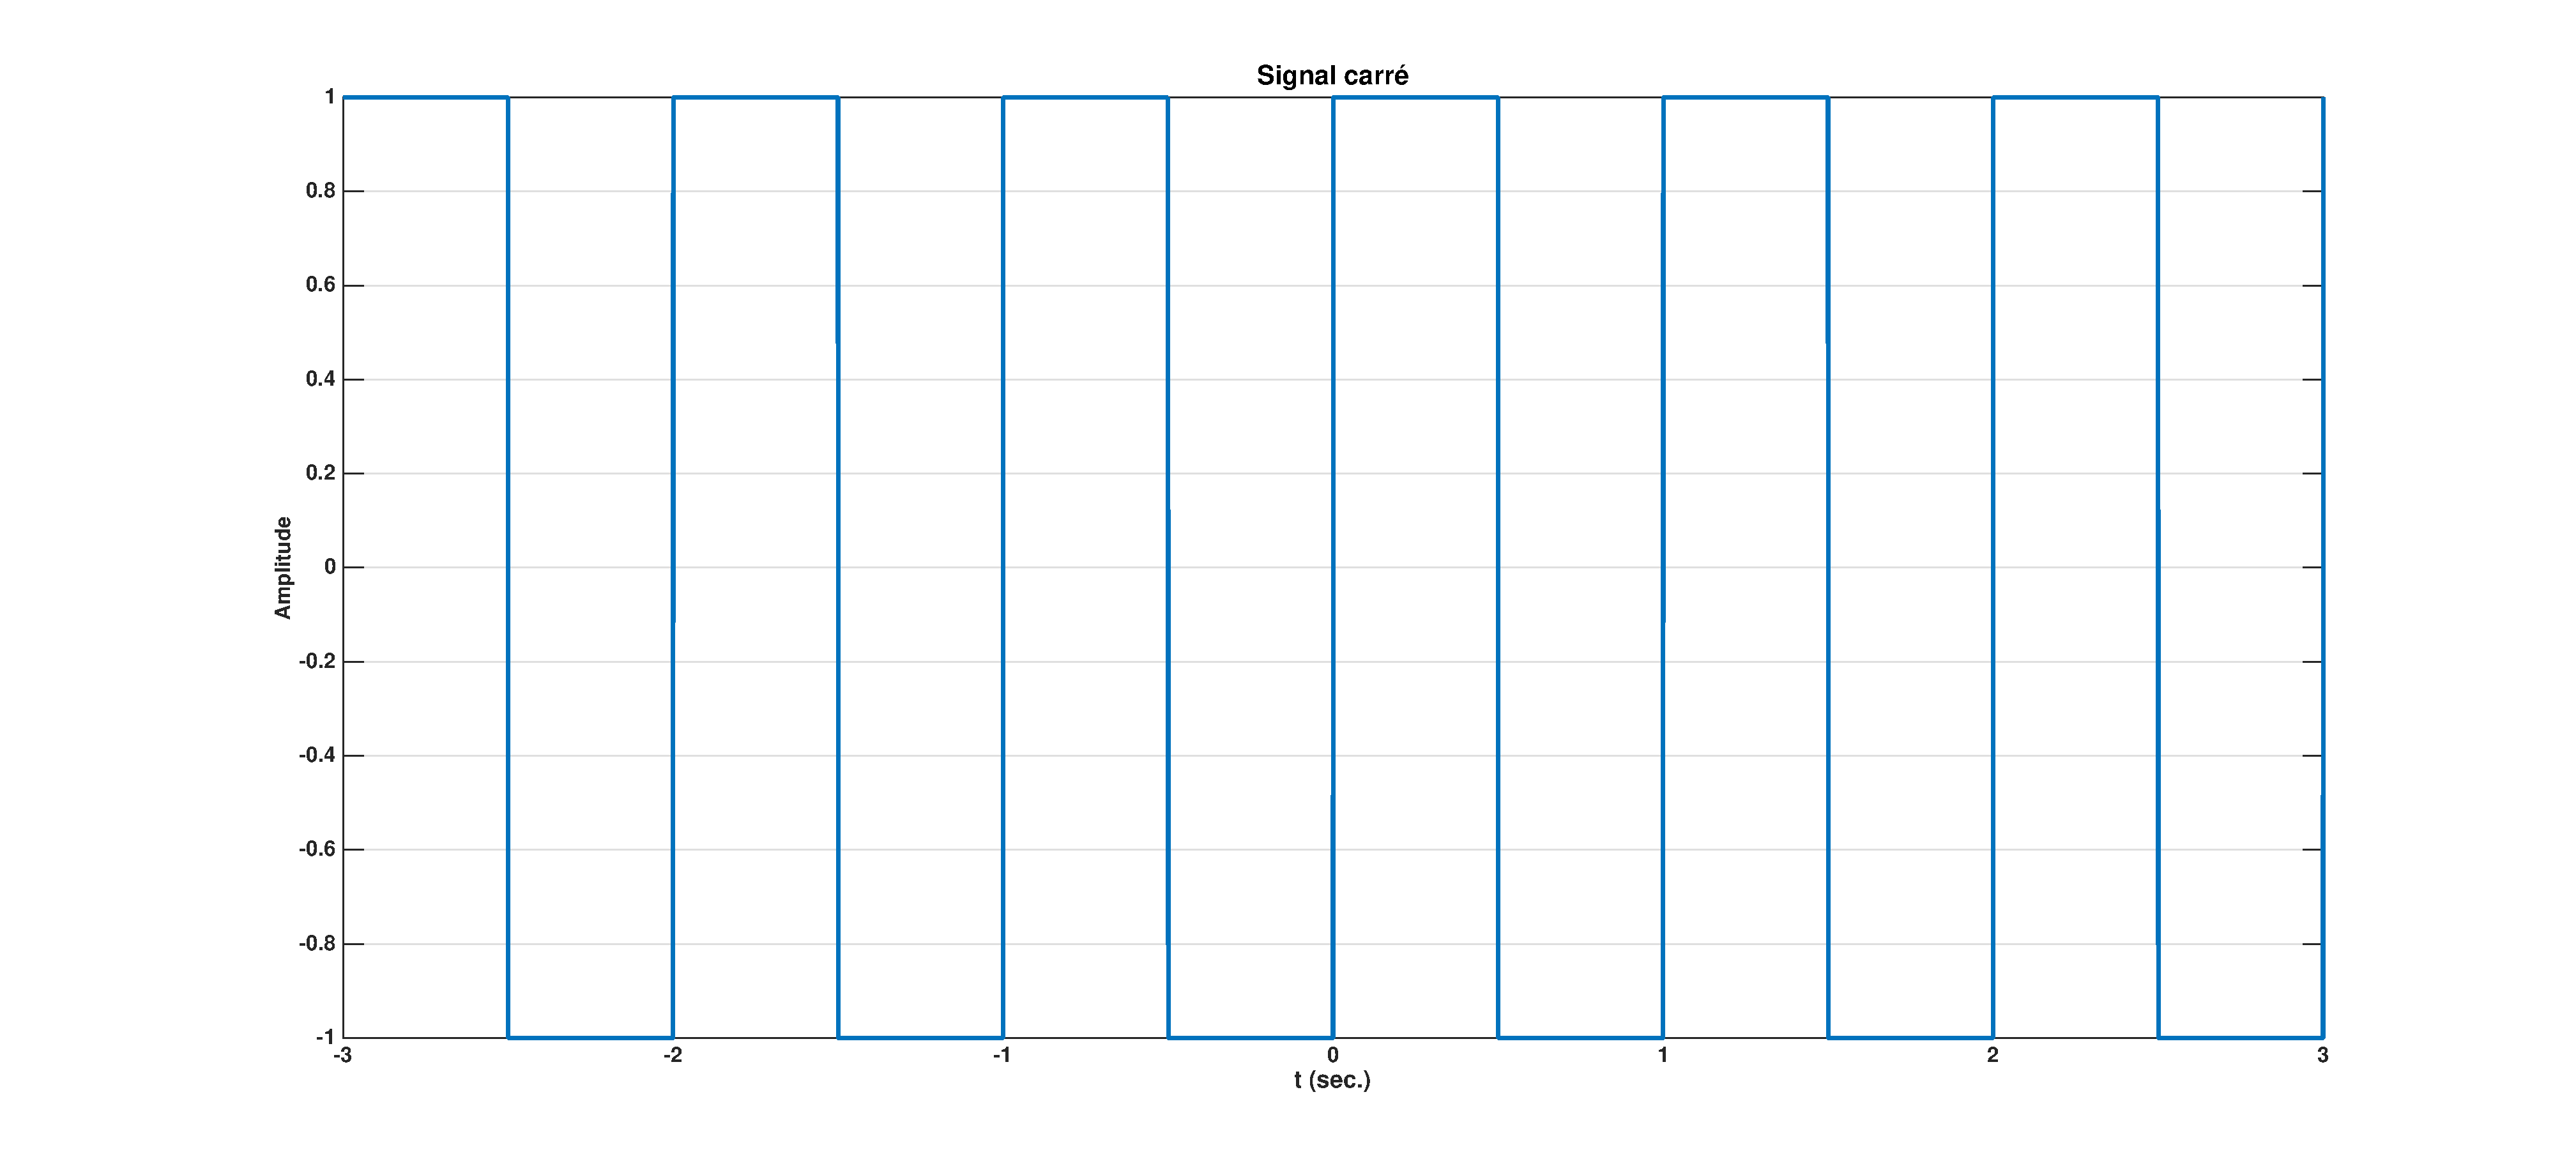
\includegraphics[scale=0.15]{Matlab/SignalCarre.eps}
\end{exampleblock}
\end{frame}
 
\end{document}
